\emph{Pour $t \in [0~;~5]$, $f(t) = \dfrac{4t+1}{\e^t}$ où $t$ est le temps en heures écoulé
depuis le décollage et $f(t)$ l'altitude de la montgolfière en kilomètres, par rapport au
niveau de la mer.}

\begin{enumerate}
	\item Le décollage correspond à $t = 0$ :
	\[f(0) = \dfrac{4 \times 0 + 1}{\e^0} = \dfrac{1}{1} = 1.\]
	Au décollage, la montgolfière est à 1~km d'altitude : c'est l'altitude du village de
	montagne.

	\item $f$ est un quotient $\dfrac{u}{v}$ avec $u(t) = 4t + 1$, $u'(t) = 4$ et $v(t) = \e^t$, $v'(t) = \e^t$
	($v$ ne s'annule pas). Pour tout réel $t$ de $[0~;~5]$ :
	\[f'(t) = \dfrac{4\e^t - (4t+1)\e^t}{\left(\e^t\right)^2}
	= \dfrac{\e^t\left(4 - 4t - 1\right)}{\e^t \times \e^t}
	= \dfrac{3 - 4t}{\e^t}.\]

	\item Pour tout réel $t$, $\e^t > 0$ : le signe de $f'(t)$ est celui de son numérateur $3 - 4t$.

	Or $3 - 4t \geqslant 0 \iff -4t \geqslant -3 \iff t \leqslant \dfrac{3}{4}$.

	\begin{center}
		\begin{tikzpicture}
			\tkzTabInit[lgt=3.4,espcl=2.8]
			{$t$/0.9,$3-4t$/0.8,$\e^t$/0.8,$f'(t)$/0.8,$f$/2.2}{$0$,$\dfrac{3}{4}$,$5$}
			\tkzTabLine{,+,z,-,}
			\tkzTabLine{,+,,+,}
			\tkzTabLine{,+,z,-,}
			\tkzTabVar{-/$1$,+/$\dfrac{4}{\e^{3/4}}$,-/$\dfrac{21}{\e^5}$}
		\end{tikzpicture}
	\end{center}

avec $f(0)=1$ d'après la question 1 et $f(5)=\frac{4\times 5 + 1}{e^5} = \frac{21}{e^5}$.

	$f'(t) > 0$ sur $\left[0~;~\dfrac{3}{4}\right[$, $f'\left(\dfrac{3}{4}\right) = 0$ et
	$f'(t) < 0$ sur $\left]\dfrac{3}{4}~;~5\right]$. La fonction $f$ est donc croissante sur
	$\left[0~;~\dfrac{3}{4}\right]$ puis décroissante sur $\left[\dfrac{3}{4}~;~5\right]$ : elle
	admet un \textbf{maximum en} $\boldsymbol{t = \dfrac{3}{4}}$, égal à
	$f\left(\dfrac{3}{4}\right) = \dfrac{4}{\e^{3/4}}$.

	\item La montgolfière perd de l'altitude dès que $f$ devient décroissante, c'est-à-dire à partir de $t = \dfrac{3}{4}$~h.
	
Or $\dfrac{3}{4} \times 60 = 45$ : la montgolfière monte pendant 45~minutes après le
	décollage.

10~h~50~min $+$ 45~min $=$ 10~h~95~min $=$ 11~h~35~min.

La montgolfière commence à perdre de l'altitude à \textbf{11~h~35}, soit 45~minutes
	après son décollage.
\end{enumerate}
